\documentclass[PI,LAB]{HSEUniversity}

\usepackage{graphicx}
\graphicspath{ {img/} }

\usepackage{hyperref}
\hypersetup{
    colorlinks=true,
    linkcolor=black,
    filecolor=magenta,      
    urlcolor=cyan,
}

\title{Организация паттернов проектирования. Порождающие паттерны Абстрактная фабрика и Одиночка}
\author{Рязанов Иван Дмитриевич}
\supervisor{к.т.н., доцент кафедры Информационных технологий в бизнесе НИУ ВШЭ-Пермь}{А.В.~Кычкин}
\Year{2020}

\begin{document}
\maketitle
\chapter{Абстрактная фабрика}
\textbf{Название и классификация паттерна.}
Абстрактная фабрика - паттерн, порождающий объекты.

\textbf{Назначение.}
Предоставляет интерфейс для создания семейств взаимосвязанных или взаимозависимых объектов, без указания их конкретных классов.

\textbf{Применимость.}
Использование паттерна Abstract Factory (абстрактная фабрика) целесообразно если:
\begin{itemize}
  \item система не должна зависеть от того, как создаются, компонуются и представляются входящие в нее объекты;
  \item входящие в семейство взаимосвязанные объекты должны использоваться вместе и вам необходимо обеспечить выполнение этого ограничения;
  \item система должна конфигурироваться одним из семейств составляющих ее объектов, а вы хотите предоставить библиотеку объектов, раскрывая только их интерфейсы, но не реализацию.
\end{itemize}
\clearpage

\begin{figure}[p]
  \centering
  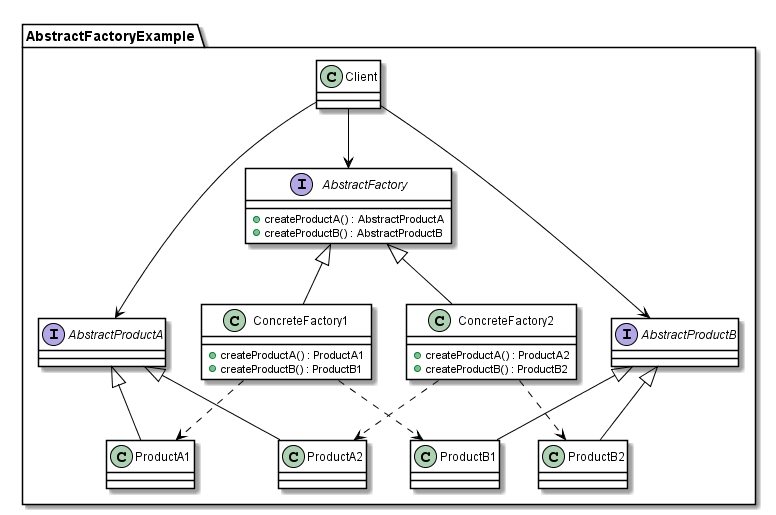
\includegraphics[scale=0.6]{AF_CD.png}
  \caption{Диаграмма классов паттерна <<Абстрактная фабрика>>}
\end{figure}

\begin{figure}[p]
  \centering
  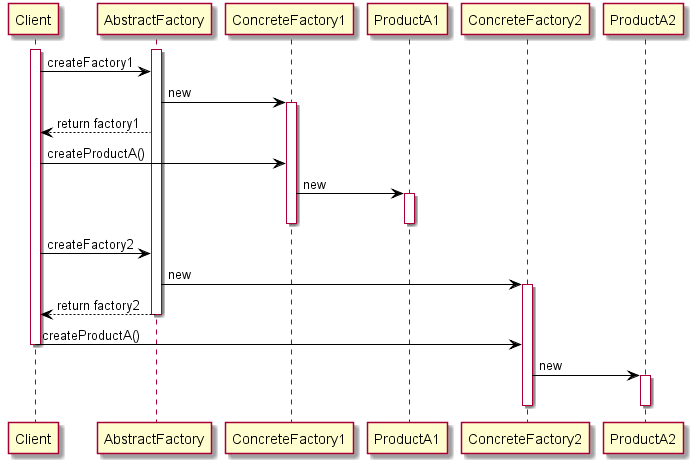
\includegraphics[scale=0.6]{AF_SD.png}
  \caption{Диаграмма последовательности паттерна <<Абстрактная фабрика>>}
\end{figure}
\clearpage

\textbf{Участники}
\begin{itemize}
  \item AbstractFactory - абстрактная фабрика: объявляет интерфейс для операций, создающих абстрактные объекты-продукты;
  \item ConcreteFactory (ConcreteFactory1, ConcreteFactory2) - конкретная фабрика: реализует операции, создающие конкретные объекты-продукты;
  \item AbstractProduct (AbstractProductА, AbstractProductВ) - абстрактный продукт: объявляет интерфейс для типа объекта-продукта;
  \item ConcreteProduct (ProductА, ProductВ) - конкретный продукт: определяет объект-продукт, создаваемый соответствующей конкретной - реализует интерфейс Abstract Product;
  \item Client - клиент: пользуется исключительно интерфейсами, которые объявлены в классах AbstractFactory и AbstractProduct.
\end{itemize}

\textbf{Отношения}
\begin{itemize}
  \item Обычно во время выполнения создается единственный экземпляр класса ConcreteFactory. Эта конкретная фабрика создает объекты-продукты, имеющие вполне определенную реализацию. Для создания других видов объектов клиент должен воспользоваться другой конкретной фабрикой;
  \item AbstractFactory передоверяет создание объектов-продуктов своему подклассу ConcreteFactory.
\end{itemize}

\textbf{Плюсы и минусы.}

Плюсы:
\begin{itemize}
  \item \textit{изолирует конкретные классы.} Помогает контролировать классы объектов, создаваемых приложением. Поскольку фабрика инкапсулирует ответственность за создание классов и сам процесс их создания, то она изолирует клиента от деталей реализации классов. Клиенты манипулируют экземплярами через их абстрактные интерфейсы. Имена изготавливаемых классов известны только конкретной фабрике, в коде клиента они не упоминаются;
  \item \textit{упрощает замену семейств продуктов.} Класс конкретной фабрики появляется в приложении только один раз: при инстанцировании. Это облегчает замену используемой приложением конкретной фабрики. 
  \item \textit{гарантирует сочетаемость продуктов.} Если продукты некоторого семейства  спроектированы для совместного использования, то важно, чтобы приложение в каждый момент времени работало только с продуктами единственного семейства. Класс AbstractFactory позволяет легко соблюсти это ограничение;
\end{itemize}
Минусы:
\begin{itemize}
  \item \textit{поддержать новый вид продуктов трудно.} Расширение абстрактной фабрики для изготовления новых видов продуктов - непростая задача. Интерфейс AbstractFactory фиксирует набор продуктов, которые можно создать. Для поддержки новых продуктов необходимо расширить интерфейс фабрики, то есть изменить класс AbstractFactory и все его подклассы.
\end{itemize}

\textbf{Области применения}

\begin{enumerate}
  \item Создание кроссплатформенных интерфейсов.
  \item Класс для работы с разными СУБД.
\end{enumerate}

\chapter{Одиночка}
\textbf{Название и классификация паттерна.}
Одиночка - паттерн, порождающий объекты.

\textbf{Назначение.}
Гарантирует, что у класса есть только один экземпляр, и предоставляет к нему глобальную точку доступа.

\textbf{Применимость.}
Использование паттерна Singleton (одиночка) целесообразно если:
\begin{itemize}
  \item должен быть ровно один экземпляр некоторого класса, легко доступный всем клиентам;
  \item единственный экземпляр должен расширяться путем порождения подклассов, и клиентам нужно иметь возможность работать с расширенным экземпляром без модификации своего кода.
\end{itemize}
\clearpage

\begin{figure}[p]
  \centering
  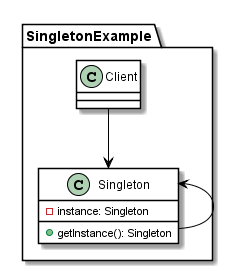
\includegraphics[scale=1]{Singleton_CD.png}
  \caption{Диаграмма классов паттерна <<Одиночка>>}
\end{figure}

\begin{figure}[p]
  \centering
  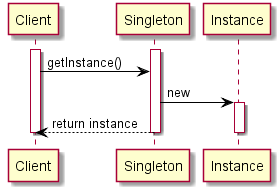
\includegraphics[scale=1]{Singleton_SD.png}
  \caption{Диаграмма последовательности паттерна <<Одиночка>>}
\end{figure}
\clearpage

\textbf{Участники}

Singleton - одиночка:
\begin{itemize}
  \item определяет операцию getInstance, которая позволяет клиентам получать доступ к единственному экземпляру;
  \item может нести ответственность за создание собственного уникального экземпляра.
\end{itemize}

\textbf{Отношения}

Клиенты получают доступ к экземпляру класса Singleton только через его операцию getInstance.

\textbf{Плюсы и минусы.}

Плюсы:
\begin{itemize}
  \item \textit{контролируемый доступ к единственному экземпляру.} Поскольку класс Singleton инкапсулирует свой единственный экземпляр, он полностью контролирует то, как и когда клиенты получают доступ к нему;
  \item \textit{уменьшение числа имен.} Паттерн одиночка - шаг вперед по сравнению с глобальными переменными. Он позволяет избежать засорения пространства имен глобальными переменными, в которых хранятся уникальные экземпляры;
  \item \textit{допускает уточнение операций и представления.} От класса Singleton можно порождать подклассы, а приложение легко сконфигурировать экземпляром расширенного класса. Можно конкретизировать приложение экземпляром того класса, который необходим во время выполнения;
  \item \textit{допускает переменное число экземпляров.} Паттерн позволяет вам легко изменить свое решение и разрешить появление более одного экземпляра класса Singleton. Вы можете применять один и тот же подход для управления числом экземпляров, используемых в приложении. Изменить нужно будет лишь операцию, дающую доступ к экземпляру класса Singleton;
\end{itemize}
Минусы:
\begin{itemize}
  \item глобальные объекты могут быть вредны для объектного программирования, в некоторых случаях приводят к созданию немасштабируемого проекта;
  \item усложняет написание модульных тестов и следование TDD;
  \item усложняется контроль за межпоточными гонками и задержками.
\end{itemize}

\textbf{Области применения}

\begin{enumerate}
  \item Ведение отладочного файла для приложения.
  \item Класс для подключения к СУБД.
\end{enumerate}

\chapter{Проектирование и реализация}
\section{Проектирование}
Для реализации был выбран 4 вариант: 

<<Приложение с поддержкой графического интерфейса пользователя рассчитано на использование на различных платформах мобильных устройств, при этом внешний вид этого интерфейса должен соответствовать принятому стилю для той или иной платформы. Например, если это приложение установлено на iOS, то его кнопки, меню, полосы прокрутки должны отображаться в стиле, принятом для приложений iOS. Группой взаимосвязанных объектов в этом случае будут элементы графического интерфейса для конкретной платформы.>>

Перед началом работы построим диаграмму классов.
\begin{figure}[h]
  \centering
  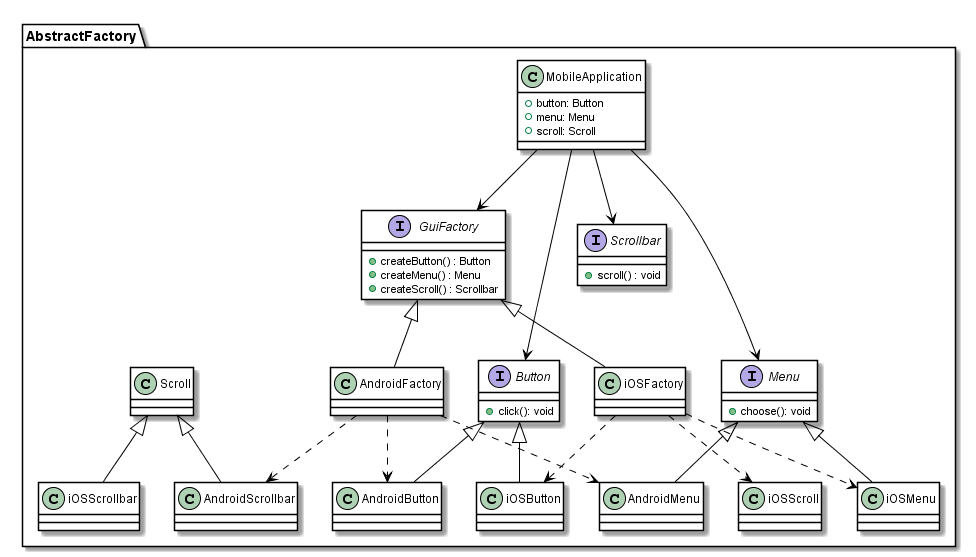
\includegraphics[scale=0.5]{Task_CD.png}
  \caption{Диаграмма классов}
\end{figure}

\textbf{Участники.}
\begin{itemize}
  \item GuiFactory - абстрактная фабрика: объявляет интерфейс для операций, создающих абстрактные кнопки, меню и скроллбары;
  \item iOSFactory, AndroidFactory - фабрики для систем iOS и Android: реализует операции, создающие конкретные элементы интерфейса;
  \item Button, Menu, Scrollbar - абстрактный элементы интерфейса: объявляют интерфейс для типа объекта-продукта;
  \item iOSButton, iOSMenu, iOSScrollbar, AndroidButton, AndroidMenu, AndroidScrollbar - конкретные реализации элементов интерфейса: определяют объекты-продукты, создаваемые соответствующей конкретной фабрикой - реализуют интерфейсы Button, Menu, Scrollbar;
  \item MobileApplication - клиент: пользуется исключительно интерфейсами, которые объявлены в классах GuiFactory, Button, Menu, Scrollbar.
\end{itemize}

\section{Реализация}
Было реализовано 2 версии программы:
\begin{enumerate}
  \item Реализация паттерна <<Абстрактная фабрика>> \href{https://github.com/rovany706/design-patterns/tree/Abstract-factory/AbstractFactoryAndSingleton/src/ru/ryazanov/HSE}{github.com}
  \item Модификация первой программы, путем добавления класса-одиночки  \href{https://github.com/rovany706/design-patterns/tree/master/AbstractFactoryAndSingleton/src/ru/ryazanov/HSE}{github.com}
\end{enumerate}

\end{document}